% This is samplepaper.tex, a sample chapter demonstrating the
% LLNCS macro package for Springer Computer Science proceedings;
% Version 2.21 of 2022/01/12
%
\documentclass[runningheads]{llncs}
%
\usepackage[T1]{fontenc}
% T1 fonts will be used to generate the final print and online PDFs,
% so please use T1 fonts in your manuscript whenever possible.
% Other font encondings may result in incorrect characters.
%
\usepackage{graphicx}
% Used for displaying a sample figure. If possible, figure files should
% be included in EPS format.
%
\usepackage{amsmath}
\usepackage{amssymb}
\usepackage{booktabs}
\usepackage{tabularx}
\usepackage[hidelinks,breaklinks=true]{hyperref}
\setlength{\emergencystretch}{2em}
%
% If you use the hyperref package, please uncomment the following two lines
% to display URLs in blue roman font according to Springer's eBook style:
%\usepackage{color}
%\renewcommand\UrlFont{\color{blue}\rmfamily}
%\urlstyle{rm}
%
\begin{document}
%
\title{Stockrium: A Tool for Financial Strategy Experimentation}
%
\titlerunning{Stockrium: A Tool for Financial Strategy Experimentation}
% If the paper title is too long for the running head, you can set
% an abbreviated paper title here
%
\author{Vinh Khang NGUYEN\inst{1}\orcidID{0009-0002-4688-0819} \and
Quoc Huy LE\inst{1}\orcidID{0009-0004-4393-1056} \and
Thi Minh Tuyen NGUYEN\inst{1}\orcidID{0000-0002-2260-4513}}
%
\authorrunning{N. V. Khang et al.}
% First names are abbreviated in the running head.
% If there are more than two authors, 'et al.' is used.
%
\institute{
  University of Science, Ho Chi Minh City National University,
  227 Nguyen Van Cu Street, District 5, Ho Chi Minh City 700000, Vietnam\\
  \email{22125035@student.hcmus.edu.vn}\\
  \email{22125031@student.hcmus.edu.vn}\\
  \email{ntmtuyen@fit.hcmus.edu.vn}
}
%
\maketitle              % typeset the header of the contribution
%
\begin{abstract}
Vietnam's stock market is among the most retail-driven in the region, yet
ordinary investors must reconcile technical, fundamental and news signals across
fragmented, largely English-centric tools. We present \emph{Stockrium}, an
agentic decision-support system for Vietnamese equities that unifies these signals
with recommendation generation. For live analysis, its current LangGraph pipeline
uses a deterministic orchestrator to dispatch technical evidence together with the
configured fundamental and news branches in parallel, then combines their normalized
scores in a deterministic buy/wait gate. Language models explain the technical evidence,
interpret and score fundamental and news evidence, summarize the decision, and
propose a trading plan only after a buy; Python calculates technical signals,
applies the weighted decision thresholds and validates horizon-dependent risk
bounds against the plan's reference price. Users can toggle the news and fundamental
sources, select at least one technical indicator and set source weights. The medium-term backtest instead uses
a sequential historical adapter over the same agent functions. In a reported
three-year VN30\footnote{VN30: the index of the $30$ largest and most-liquid stocks
on the Ho Chi Minh Stock Exchange (HOSE).} backtest, the pipeline produced $64.0\%$
fewer completed trades and a realized-trade drawdown statistic that was $9.93$
percentage points smaller than its technical-engine comparator. Although these
figures show greater selectivity and a smaller recorded drawdown statistic, they
also show lower median return and win rate. The system is decision-support only and
confined to Vietnamese equities.

\keywords{Agentic AI \and Large language models \and Multi-agent systems \and
Investment decision support \and Vietnamese
stock market}
\end{abstract}
%
%
%
% ============================================================
% Section 1 — Introduction
% ============================================================
\section{Introduction}
\label{sec:introduction}

Vietnam's stock market has a large retail base: by the end of 2025 domestic
investors held about $11.9$ million securities accounts (some $11.6\%$ of the
population) and around $90\%$ of daily trading
value~\cite{vsd2025,vinacapital2024}. FTSE Russell confirmed in April 2026 that
Vietnam will become a Secondary Emerging market in September
2026~\cite{ftse2026}. Yet domestic investors have been shown to follow foreign
trading~\cite{vnherd2022}; non-professionals forming much of the volume lack
experience, are prone to losses~\cite{barber2013}, and can be influenced by online
opinion leaders and fear of missing out~\cite{vnfomo}.

Market applications expose charts, company data, news and commentary, but these
lenses often remain split across screens and workflows. What is needed is a tool
that reconciles them in Vietnamese and returns a clear recommendation whose
inputs and thresholds can be inspected and tested. An unconstrained LLM is a poor
fit when real money is at stake because its numerical decisions are hard to
reproduce. Stockrium therefore separates semantic interpretation from measurable
controls: the model produces typed analyses and, after a buy decision, a candidate
trading plan, while Python owns planning, technical scoring, the weighted buy gate
and final validation of the plan.

We present \emph{Stockrium}, whose live-analysis path is a LangGraph pipeline for
Vietnamese equities. A deterministic orchestrator fans out to the
always-enabled technical branch and the optionally enabled fundamental and news
branches; each branch separates data
preparation from interpretation. A recommendation node computes the weighted score
and buy/wait result, generates and validates risk targets for a buy, and passes the
immutable decision to a final summarizer. The user can toggle news and fundamental
branches, choose technical indicators and supply validated source weights. A
separate internal web interface gives authorized evaluators a chart-based testbed
for controlled analysis and historical backtesting. The backtest path reuses the
production agent functions through a sequential historical adapter.

This paper makes the following contributions:
\begin{itemize}
\item A configurable LangGraph-based decision-support system that integrates
technical, fundamental and news evidence, separates data preparation from LLM
interpretation, applies explicit scoring and risk-validation rules, and helps users
inspect recommendations by selecting data sources, technical indicators and source
weights.
\item A purpose-built Vietnamese backtesting tool whose sequential
historical adapter reuses the production agents, overlays trades on the price chart
and evaluates strategies with significance testing.
\item A prototype Vietnamese dataset covering price and volume history, company
fundamentals, and stock-linked news with stored summaries and sentiment labels.
\end{itemize}

\paragraph{Scope.}
The system is \emph{decision-support} only: it produces analysis and
recommendations but does \emph{not} execute orders, connect to a brokerage, or
manage portfolios, and its output is not financial advice. Its coverage is
confined to Vietnamese equities, from which all data, tickers and indices are
drawn.
\section{Related Work}
\label{sec:related}

Stockrium builds on four strands of prior work.

\emph{Multi-agent LLM systems for trading.} The closest is
TradingAgents~\cite{tradingagents}, which casts a trading firm as a society of LLM
agents---analysts, bull/bear researchers, a trader and a risk team---that
communicate through structured outputs and natural-language debate, reporting gains
on US equities over single-agent and rule baselines. Its role specialization and
structured communication inform our design, but it runs on US-centric data and lets
the agents debate their way to the decision, which is costly and sensitive to
prompt and sampling variation. FinMem~\cite{finmem} instead gives a single LLM
trader a layered memory; like TradingAgents, it keeps the decision inside the
model. Stockrium adapts the multi-agent idea to the Vietnamese market but separates
LLM-based evidence scoring from a deterministic recommendation rule and adds
per-source and per-indicator configuration.

\emph{Finance-specific LLMs.} BloombergGPT~\cite{bloomberggpt} and the open-source
FinGPT~\cite{fingpt} improve financial NLP such as sentiment classification and
summarization, but they are analytical \emph{assistants}: they neither fuse
multiple lenses nor produce risk-managed, backtested recommendations, and none
targets Vietnamese equities. We therefore use a strong general model for the
language tasks and build the decision logic around it.

\emph{Financial news sentiment analysis.} FinBERT and its
successors~\cite{finbert2023} and FinBERT-LSTM models~\cite{finbertlstm2022} turn
financial text into a sentiment signal that aids price prediction, but they are
opaque one-step predictors, not an explainable recommendation that reconciles
sentiment with technical and fundamental evidence---the role of our news agent.

\emph{The Vietnamese market.} PhoBERT-based classifiers label stock-article
sentiment well~\cite{phobertstock}, and studies report significant changes in return
variance around negative news but no statistically significant change in mean
returns~\cite{vnnews2023}; behavioural work documents herding and FOMO among newer
investors~\cite{vnherd2022,vnfomo}; for price forecasting, LSTM, BiLSTM and
Transformer models and conventional machine learning have been applied to the
VN-Index~\cite{vndl2025,vnlstm2021,vnml2024}. This work is largely single-source
and predictive, rarely LLM-based or risk-calibrated, and offers no interactive tool
for fusing signals and backtesting.

To our knowledge no prior system simultaneously (i)~unifies technical, fundamental
and news analysis with recommendation for the Vietnamese market, (ii)~uses a
hybrid LLM/rule design that stays explainable and inspectable, (iii)~enforces
horizon-dependent risk constraints, and (iv)~provides a configurable, chart-based
backtesting testbed. This paper addresses that gap.

% ============================================================
% Section 3 — System Architecture (client-server)
% ============================================================
\section{System Architecture}
\label{sec:architecture}
Stockrium follows a client-server architecture (Fig.~\ref{fig:arch}). On the
client side, a mobile application and a web application serve complementary roles.
The mobile application focuses on the core, everyday functions: displaying market
information and delivering per-stock analysis and recommendations to the user. The
web application focuses on fixed medium-term backtesting and on live analysis for
one symbol or a predefined VN30/VN100 basket. It lets authorized evaluators configure
an analysis (choosing the optional news/fundamental branches, technical indicators
and source weights), request recommendations, run a single-symbol backtest or a
sequential VN30 batch, and inspect simulated trades on the price chart. Both clients
share the same server boundary, but use different presentation technologies: the
mobile application is built with React Native and Expo, whereas the internal web
interface uses HTML, CSS and JavaScript. On the server side, a core service,
implemented with FastAPI in Python,
exposes the application's main functions through an API and coordinates the
analysis paths, persistence services and external model access. Managed Supabase
PostgreSQL stores structured market, fundamental, news and user data. Separately,
timestamped backtest visualization JSON files are uploaded to the private
\texttt{backtests} bucket in Supabase Storage and served to authorized clients
through authenticated API proxy routes. Live analysis uses the LangGraph layer
(Section~\ref{sec:framework}), whereas historical analysis uses the sequential
backtest adapter; both call an external LLM provider through the server. Keeping
thin clients separate from the server places data access, agent execution and model
credentials behind the API.

\begin{figure}[t]
\centering
\scriptsize
\setlength{\fboxsep}{5pt}
\begin{tabular}{@{}c@{\hspace{3pt}}c@{\hspace{3pt}}c@{\hspace{3pt}}c@{\hspace{3pt}}c@{}}
\fbox{\parbox[c][2.9cm][c]{0.14\textwidth}{\centering
\textbf{Clients}\\[5pt]
Mobile app\\
Admin web app}}
&
$\longleftrightarrow$
&
\fbox{\parbox[c][2.9cm][c]{0.35\textwidth}{\centering
\textbf{FastAPI server}\\[4pt]
Core service / API\\[5pt]
\texttt{/analyze}: nine-node LangGraph\\
conditional parallel branches\\[4pt]
\texttt{/backtest}: sequential adapter\\
medium-term daily agents}}
&
$\longleftrightarrow$
&
\fbox{\parbox[c][2.9cm][c]{0.25\textwidth}{\centering
\textbf{Supabase PostgreSQL}\\
market, fundamental, news, user data\\[5pt]
\rule{0.22\textwidth}{0.4pt}\\[5pt]
\textbf{Private Supabase Storage}\\
\texttt{backtests} bucket: timestamped visualization JSON}}
\end{tabular}

\vspace{4pt}
$\updownarrow$\\[-1pt]
\fbox{\parbox[c][0.8cm][c]{0.27\textwidth}{\centering
\textbf{External LLM provider}}}
\caption{Implemented client-server architecture. Structured application data
resides in PostgreSQL; backtest visualization files reside in a separate private
Supabase Storage bucket.}
\label{fig:arch}
\end{figure}

% ============================================================
% Section 4 — The Multi-Agent Framework (agents + workflow)
% ============================================================
\section{The Multi-Agent Framework}
\label{sec:framework}

For a live \texttt{/analyze} request, a nine-node LangGraph
\texttt{StateGraph} (Fig.~\ref{fig:framework}) fuses technical, fundamental and
news evidence. A deterministic orchestrator creates the technical and news time
plan. Each parallel
branch has a data-preparation node and an analysis node; the latter returns a
normalized score and narrative. A recommendation node then applies explicit
weighting and buy thresholds, and an aggregator produces the confidence and final
summary. Through \texttt{data\_selection}, users may enable or disable the news and
fundamental sources, choose at least one technical indicator and set source weights,
making the live graph configurable while keeping technical analysis mandatory.

The \texttt{/backtest} route does not invoke this compiled graph. It uses the
separate historical adapter described in Section~\ref{sec:experiments}, which
constructs an \texttt{AgentState} and calls the same production agent functions
sequentially for each prefiltered historical signal date.

\begin{figure}[t]
\centering
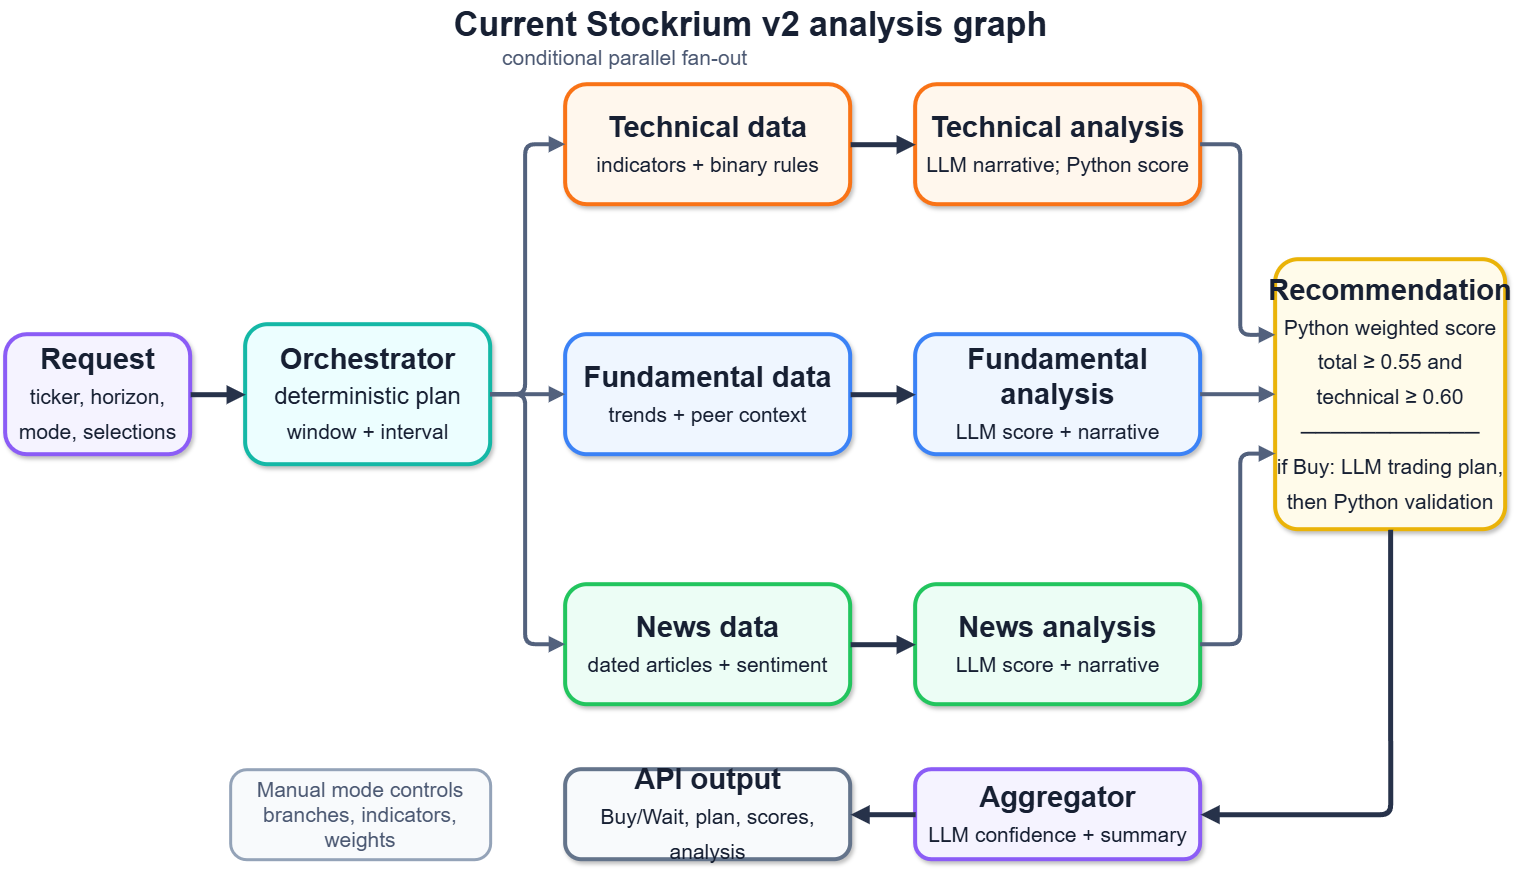
\includegraphics[width=0.9\textwidth]{fig1_framework}
\caption{The live multi-agent analysis pipeline}
\label{fig:framework}
\end{figure}

\subsection{Orchestrator Agent}
\label{sec:orchestrator}

The API schema validates field shape and ticker syntax, but does not verify that a
ticker exists on a Vietnamese exchange. The live orchestrator performs no ticker
lookup; it is fully deterministic and only maps the investor's period to fixed,
auditable windows. Missing ticker data is therefore handled later, when the
selected source agents query their stores.
Short-term analysis uses $1$-hour candles over $90$ days and news from $30$ days;
medium-term uses daily candles over $365$ days and news from $90$ days; long-term
uses weekly candles over $1{,}825$ days and news from $365$ days. Dates are
generated in the Vietnam time zone. Fundamental evidence is not assigned a
horizon-specific window by the orchestrator; it uses the latest five annual rows
available for every period. Automatic mode applies the default selection and horizon
weights, while manual mode retains the user's validated source switches, enabled
indicators and weights.

\subsection{Technical Data and Analysis Agents}
\label{sec:technical}

The technical data agent computes in NumPy/Pandas RSI ($14$), SMA ($20/50$), Bollinger
Bands ($20$, $2\sigma$), MACD ($12/26/9$) and KDJ ($9/3/3$), covering momentum,
trend, volatility/mean reversion and stochastic oscillation~\cite{murphy1999}.
Rules in Table~\ref{tab:scoring} convert each enabled indicator $i$ into a bullish
score $s_i\in\{0,1\}$, favoring fresh upward momentum over extended readings. Raw
values and a justification accompany every score. The agent reports
$S_{\mathrm{tech}}=\sum_{i\in\mathcal{E}}s_i$ and
$S_{\max}=|\mathcal{E}|$ for the user-enabled set $\mathcal{E}$ (all five by
default). The technical analysis node uses \texttt{gpt-4o-mini} only to explain the
prepared evidence; Python supplies its normalized score
$x_t=S_{\mathrm{tech}}/S_{\max}$, so the narrative cannot alter it. Live price is
kept separate from the latest OHLCV row returned within the requested period,
which is the row used for scoring. There is no explicit completed-bar check, so
for a live hourly, daily or weekly request that final row may still be forming if the
upstream source exposes it.

\begin{table}[t]
\centering
\caption{Bullish scoring rules. RSI, MA, BOLL and MACD earn $s_i=1$ if any
listed condition holds between the previous candle and the current one. KDJ
first applies its overbought veto; only otherwise can a listed bullish condition
earn one point.}
\label{tab:scoring}
\setlength{\extrarowheight}{2pt}
\renewcommand{\arraystretch}{1.0}
\begin{tabularx}{\textwidth}{@{}lX@{}}
\toprule
Indicator & Conditions for $s_i = 1$ (logical OR) \\
\midrule
RSI  & crosses above $50$; or $50\!\leq\!\mathrm{RSI}\!\leq\!70$ and rising; or $\mathrm{RSI}\!<\!35$ and rising \\
\addlinespace
MA   & golden cross (SMA20 crosses above SMA50); or SMA20$>$SMA50 with widening gap; or price$>$SMA20$>$SMA50 \\
\addlinespace
BOLL & price crosses above middle band; or above middle with increasing distance; or rebound off lower band \\
\addlinespace
MACD & crosses above signal; or MACD$>$signal with rising histogram; or histogram turns positive \\
\addlinespace
KDJ  & veto: if $K>80$, then $s_i=0$; otherwise $K$ crosses above $D$; or $K>D$ with rising $J$; or $K<20$ and rising \\
\bottomrule
\end{tabularx}
\end{table}

\subsection{Fundamental Data and Analysis Agents}
\label{sec:fundamental}

The fundamental agent reads at most the latest five annual rows from
\texttt{FA\_Indicator}. It queries the company profile only to obtain
\texttt{icb\_code}, and uses that code to load annual medians from
\texttt{FA\_Industry\_Aggregate}. The code takes the maximum \texttt{peer\_count}
among the selected annual aggregate rows and shows peer comparisons when that
maximum is at least three; it does not require every selected aggregate row to reach the
threshold. It does not load income statements,
cash-flow statements or stored narrative summaries. From the indicator rows it
computes CAGR where valid and, for non-financial firms, organizes liquidity,
leverage, efficiency, profitability and valuation evidence; DuPont components
and available industry medians provide trend and peer context. For ICB 8xxx
financial firms it instead presents the available financial-sector measures and
uses P/B rather than relying on P/E or EV/EBITDA. Missing data produces a
``no data'' evidence block rather than aborting the graph. A separate structured
LLM step assigns a score $x_f\in[0,1]$ and explanatory narrative from only this
prepared evidence.

% ============================================================
\subsection{Article Data and Analysis Agents}
\label{sec:news}

The news pipeline first stores source articles and enriches them offline with a
typed short Vietnamese summary and positive/neutral/negative sentiment, retaining
the original evidence and stock links. Online, the service first returns all linked
article records to the data node; the node then filters them to the planned interval,
sorts them by date and exposes at most the newest $50$, with date, title, a bounded
summary (falling back to description) and stored sentiment when present. The
analysis node returns a structured positivity score $x_n\in[0,1]$ and a concise
narrative. When news or fundamental evidence is disabled, its graph branch is not
executed; the aggregator consequently emits score zero and an empty source
narrative. In contrast, an enabled fundamental or news branch with no data,
or an enabled technical branch without prepared data, returns score zero with a
localized no-data explanation. If an LLM analysis call fails, fundamental and news
return zero with localized fallbacks, while technical retains its deterministic
Python score and uses a localized fallback narrative.

\subsection{Recommendation and Aggregator Agents}
\label{sec:aggregator}
The recommendation node computes
$q=w_t x_t+w_f x_f+w_n x_n$. Default
technical/fundamental/news weights are $0.60/0.10/0.30$ (short term),
$0.40/0.40/0.20$ (medium) and $0.15/0.70/0.15$ (long); manual weights are accepted
only when they sum to one. The server itself does not redistribute weights when a
source is disabled: the absent source contributes its default score of zero.
However, the first-party mobile and web configuration screens set disabled
sources to zero weight and evenly redistribute the full unit weight among enabled
sources before sending a manual request. Thus direct API requests retain their
submitted valid weights, whereas normal client-side configuration is
redistributed. The deterministic verdict is \textsf{Buy} iff $q\geq0.55$ and
$x_t\geq0.60$; otherwise it is \textsf{Wait}.

Only for \textsf{Buy}, Python sets the reference entry price to the technical
node's \texttt{current\_price}; an LLM proposes take-profit, stop-loss and holding
period within horizon-specific limits: profit/stop ranges of $8$--$15\%$/$4$--$7\%$
(short), $15$--$30\%$/$7$--$12\%$ (medium), and
$40$--$80\%$/$15$--$20\%$ (long). Python revalidates the proposal against that
reference price and a minimum reward-to-risk ratio of $1.5$; invalid or failed
plans are replaced by deterministic fallback values. In live analysis the
reference is the current matched price; in backtesting it is the signal candle's
close. Finally, the aggregator uses the LLM only for a confidence score and
summary. It cannot change the verdict or plan, and an aggregation failure is
returned as an error instead of silently fabricating a safe recommendation.
% ============================================================
% Agent Workflow (subsection of the framework section)
% ============================================================
\subsection{Agent Workflow}
\label{sec:workflow}

Figure~\ref{fig:framework} traces one live-analysis request through the shared
state, parallel branches and two-stage fusion.

\subsubsection{Shared state and communication protocol.}
The agents do not call one another directly; they communicate through a single
typed state object, \texttt{AgentState} (a \texttt{TypedDict}), that flows through
the graph. It carries the execution mode, the user input, the risk profile, the
target symbol, a \texttt{data\_selection} object (source switches, indicator
toggles and weights), the orchestrator's plan, the collected
\texttt{agent\_results}, and the final output. LLM calls use structured decoding
into Pydantic schemas rather than heuristic free-text parsing. The
\texttt{agent\_results} field is annotated with an
\texttt{operator.or\_} reducer, letting the parallel analysis agents each write
their partial result into the shared dictionary without overwriting one another.

\subsubsection{Types of agent interactions.}
Three interaction patterns compose the live pipeline. First, deterministic
planning gives the technical and news branches horizon-specific windows, while the
fundamental branch keeps its fixed five-row annual view. Second, the selected
data/analysis pairs run as parallel branches and merge through the state reducer.
Third, the recommendation node applies the weighted rule in
Section~\ref{sec:aggregator}; only afterward does the aggregator generate
presentation-level confidence and summary.

\subsubsection{Backbone LLMs.}
All LLM-backed steps use structured output from OpenAI's
\texttt{gpt-4o-mini} at temperature $0.1$. The model interprets fundamental and news
evidence, explains technical evidence, proposes a plan after a deterministic buy,
and writes the final confidence and summary. Python retains control over dates,
indicator calculation, technical normalization, weighted fusion, verdict thresholds
and plan validation. The application adds no outer retry loop, but its OpenAI
client (SDK version 2.31.0) leaves the retry setting at its default, which can
retry eligible failures up to two times. Error handling is node-specific: technical analysis
keeps its deterministic score and returns a localized fallback narrative;
fundamental and news analysis return zero with localized fallbacks; and a failed
plan-generation call produces a deterministic fallback plan. Only failure of the
final aggregator is returned as an API error.

\subsection{Implemented Interface Results}
\label{sec:interface-results}

Figure~\ref{fig:stockrium-captures} presents the implemented mobile result of the
analysis workflow. The stock-detail screen in Fig.~\ref{fig:stockrium-captures}(a)
provides the price context from which a user opens AI analysis. For a \textsf{Buy}
decision, Fig.~\ref{fig:stockrium-captures}(b) exposes the recommendation,
confidence, entry price, take-profit, stop-loss, maximum holding period and the
three component scores. Figure~\ref{fig:stockrium-captures}(c) continues with the
source-level explanation and final summary. Together, these screens demonstrate an
end-to-end implementation result: Stockrium turns the graph's structured output
into an inspectable user-facing recommendation rather than returning an unrestricted
block of model text. They demonstrate software integration and presentation, not
the financial correctness of an individual recommendation.

\begin{figure}[t]
\centering
\begin{minipage}{0.3\textwidth}
\centering
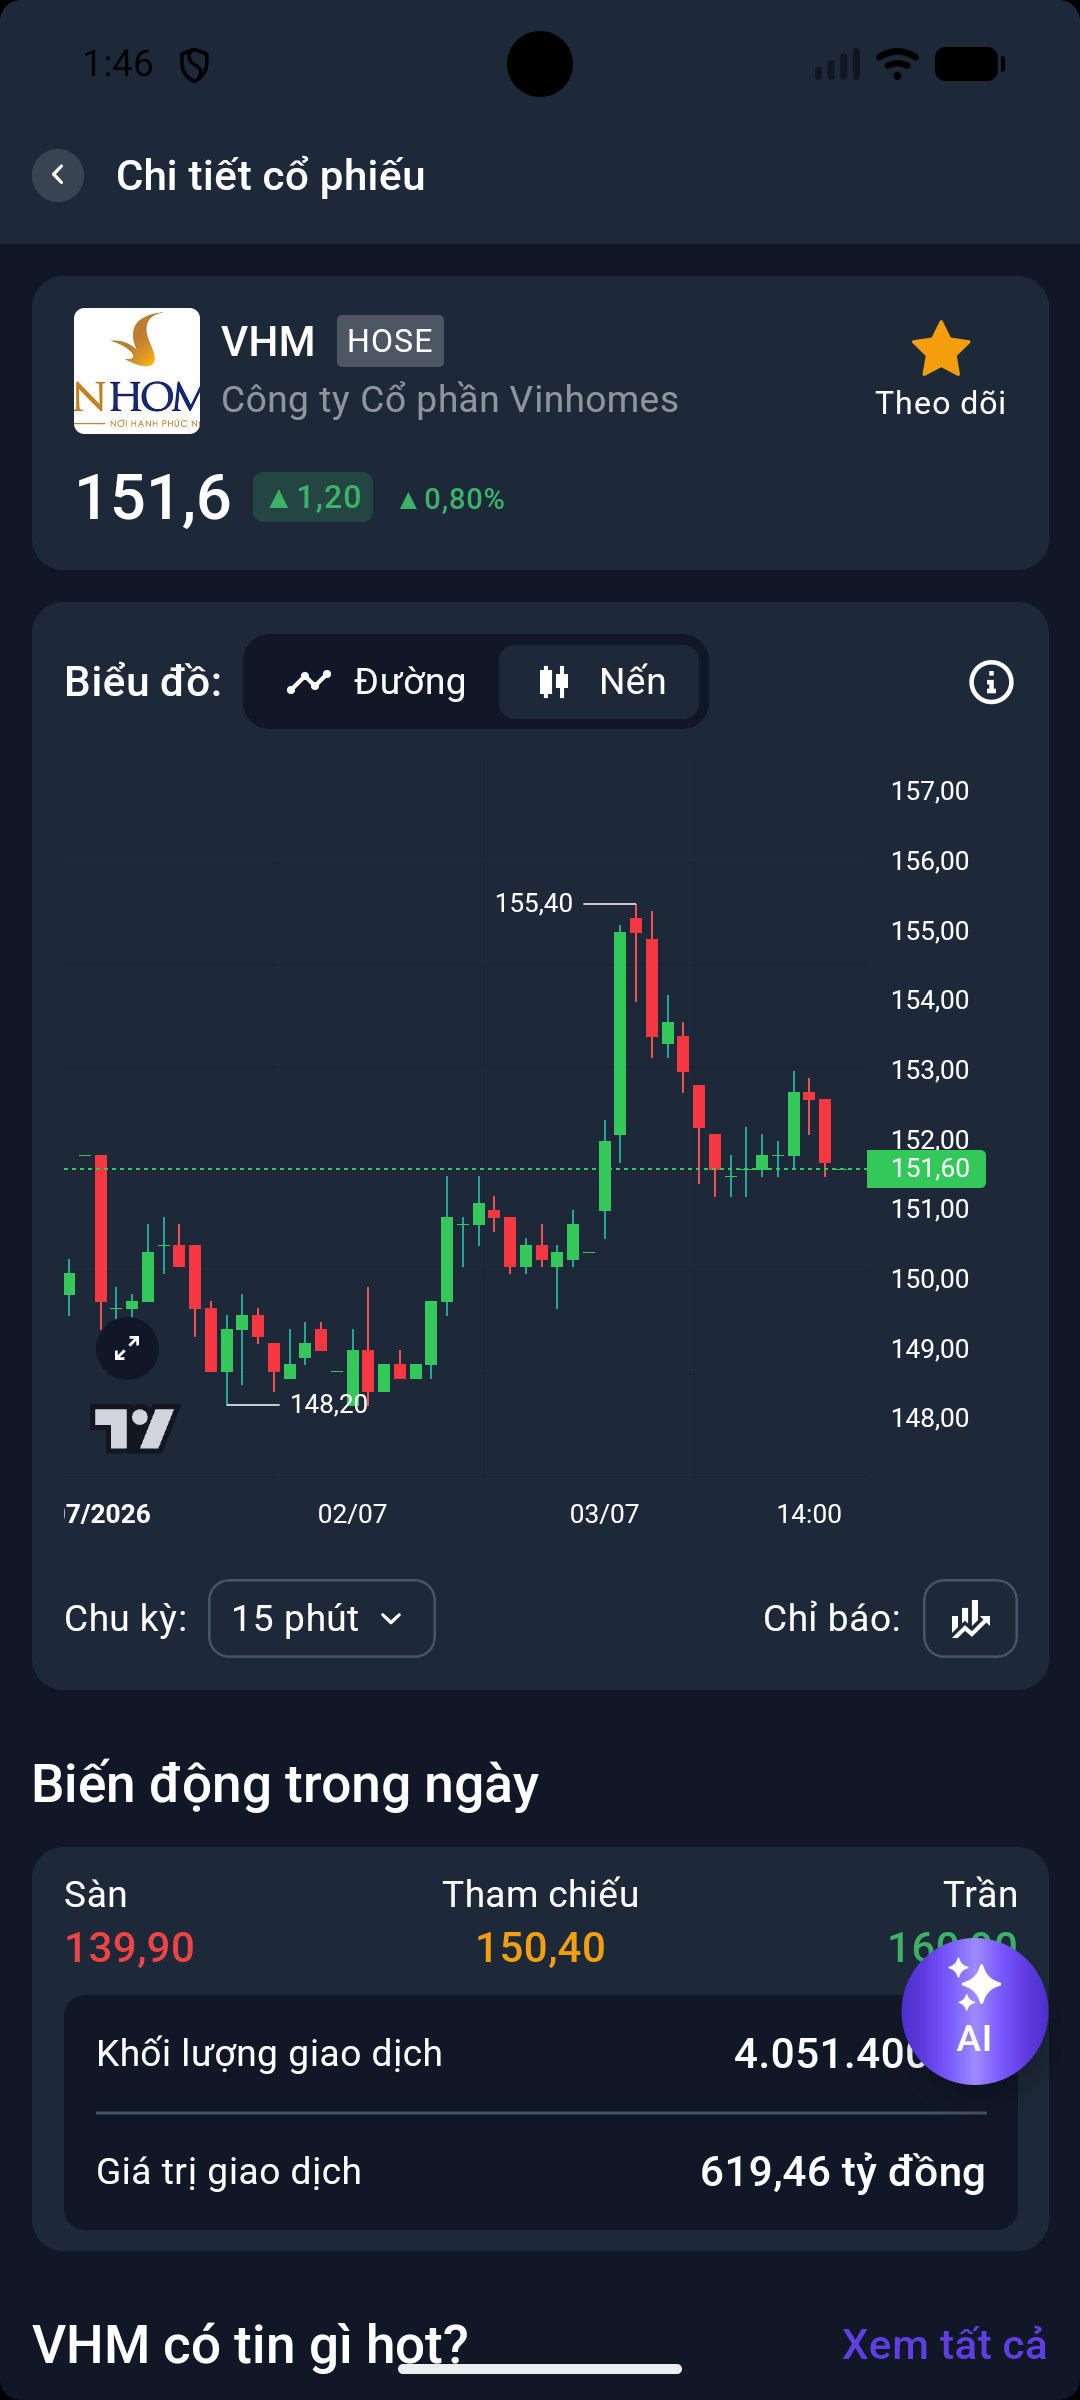
\includegraphics[width=\linewidth]{capture1.png}\\[2pt]
\footnotesize (a) Stock details and price context
\end{minipage}%
\hfill
\begin{minipage}{0.3\textwidth}
\centering
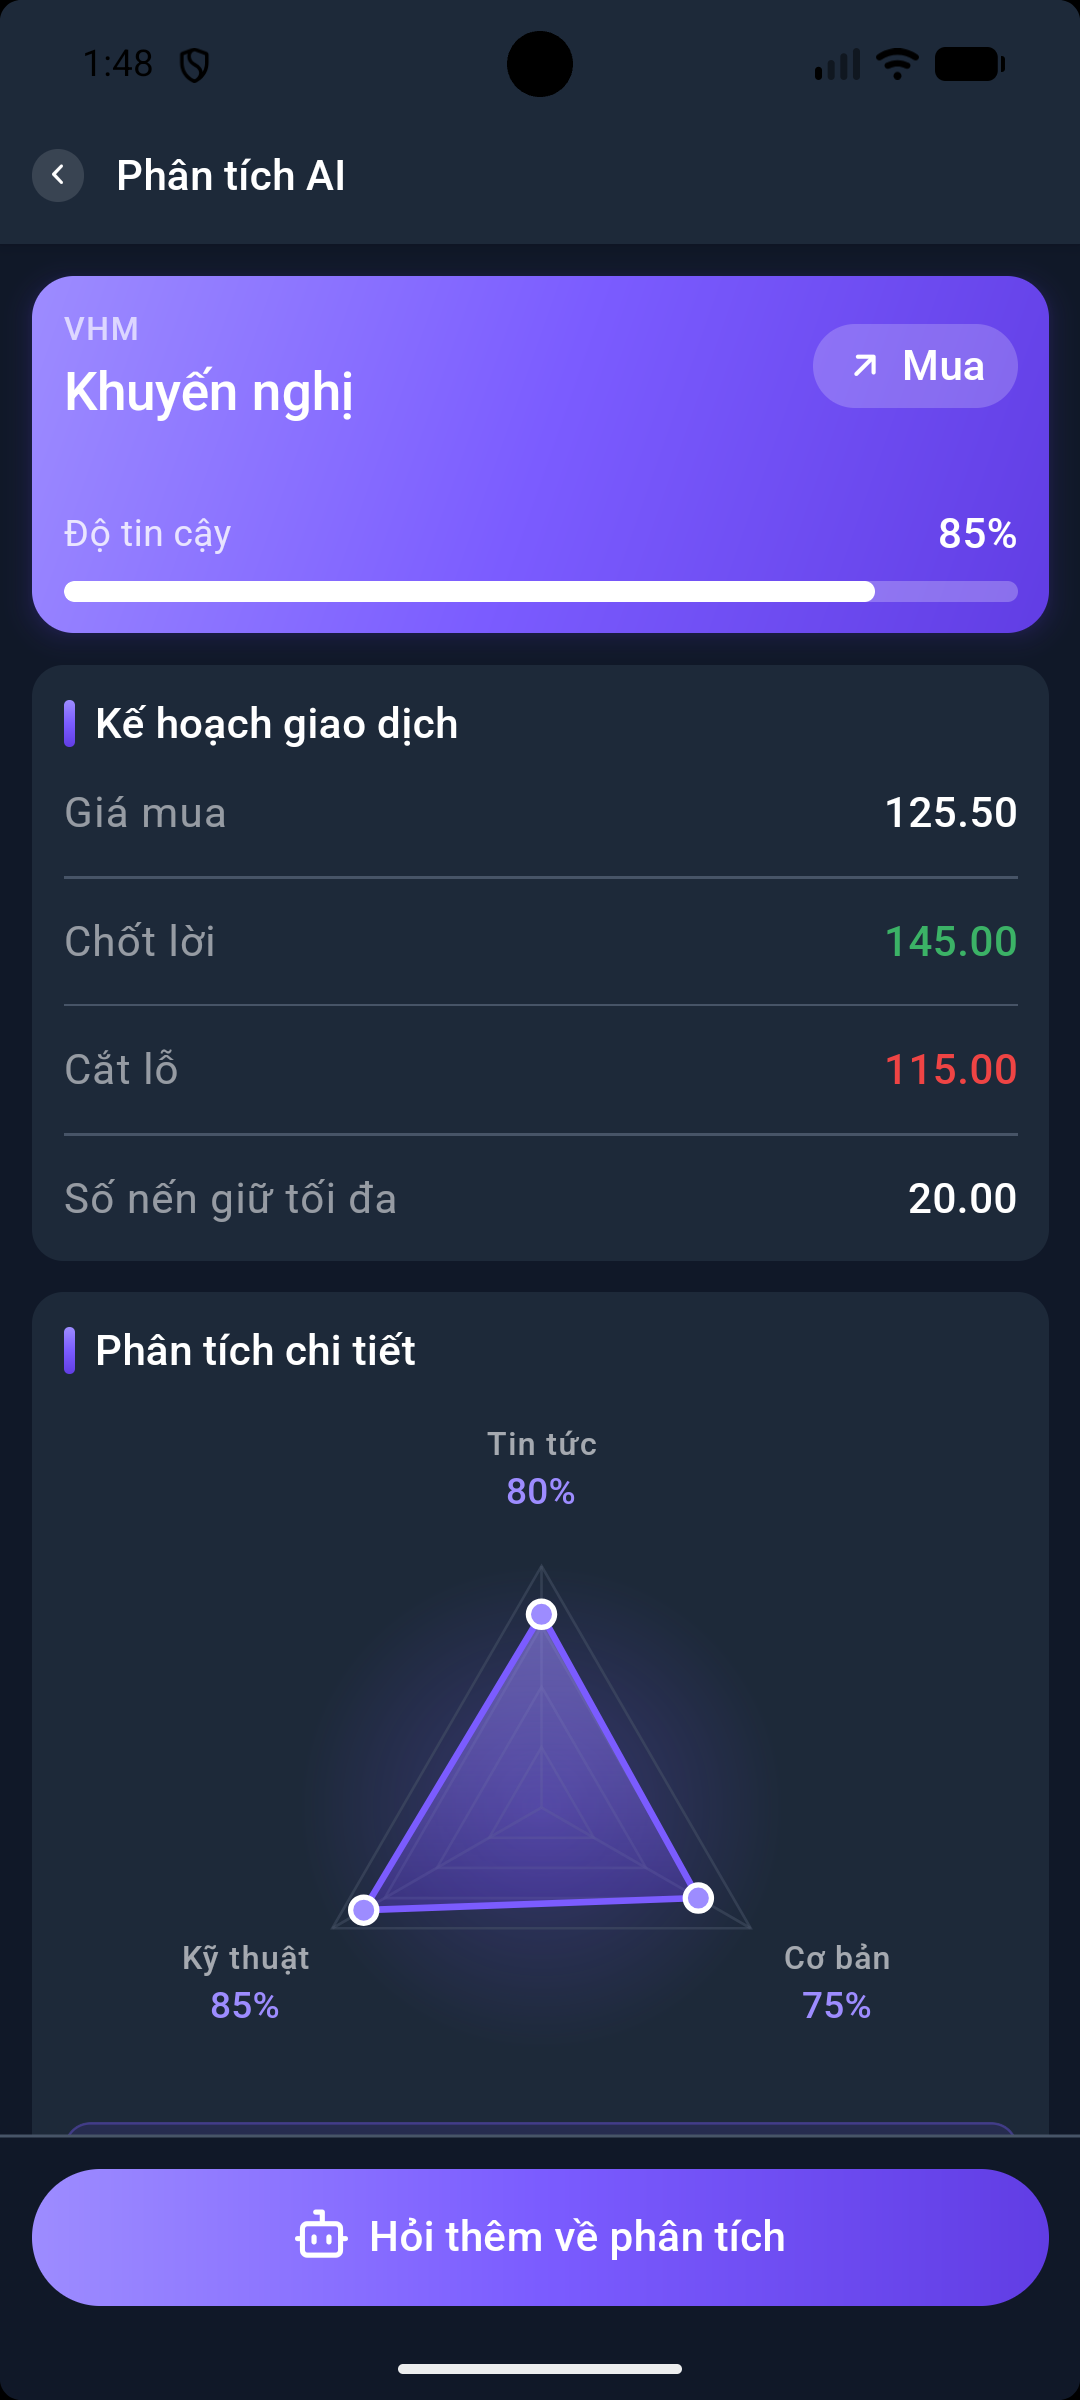
\includegraphics[width=\linewidth]{capture2.png}\\[2pt]
\footnotesize (b) Structured trading plan
\end{minipage}%
\hfill
\begin{minipage}{0.3\textwidth}
\centering
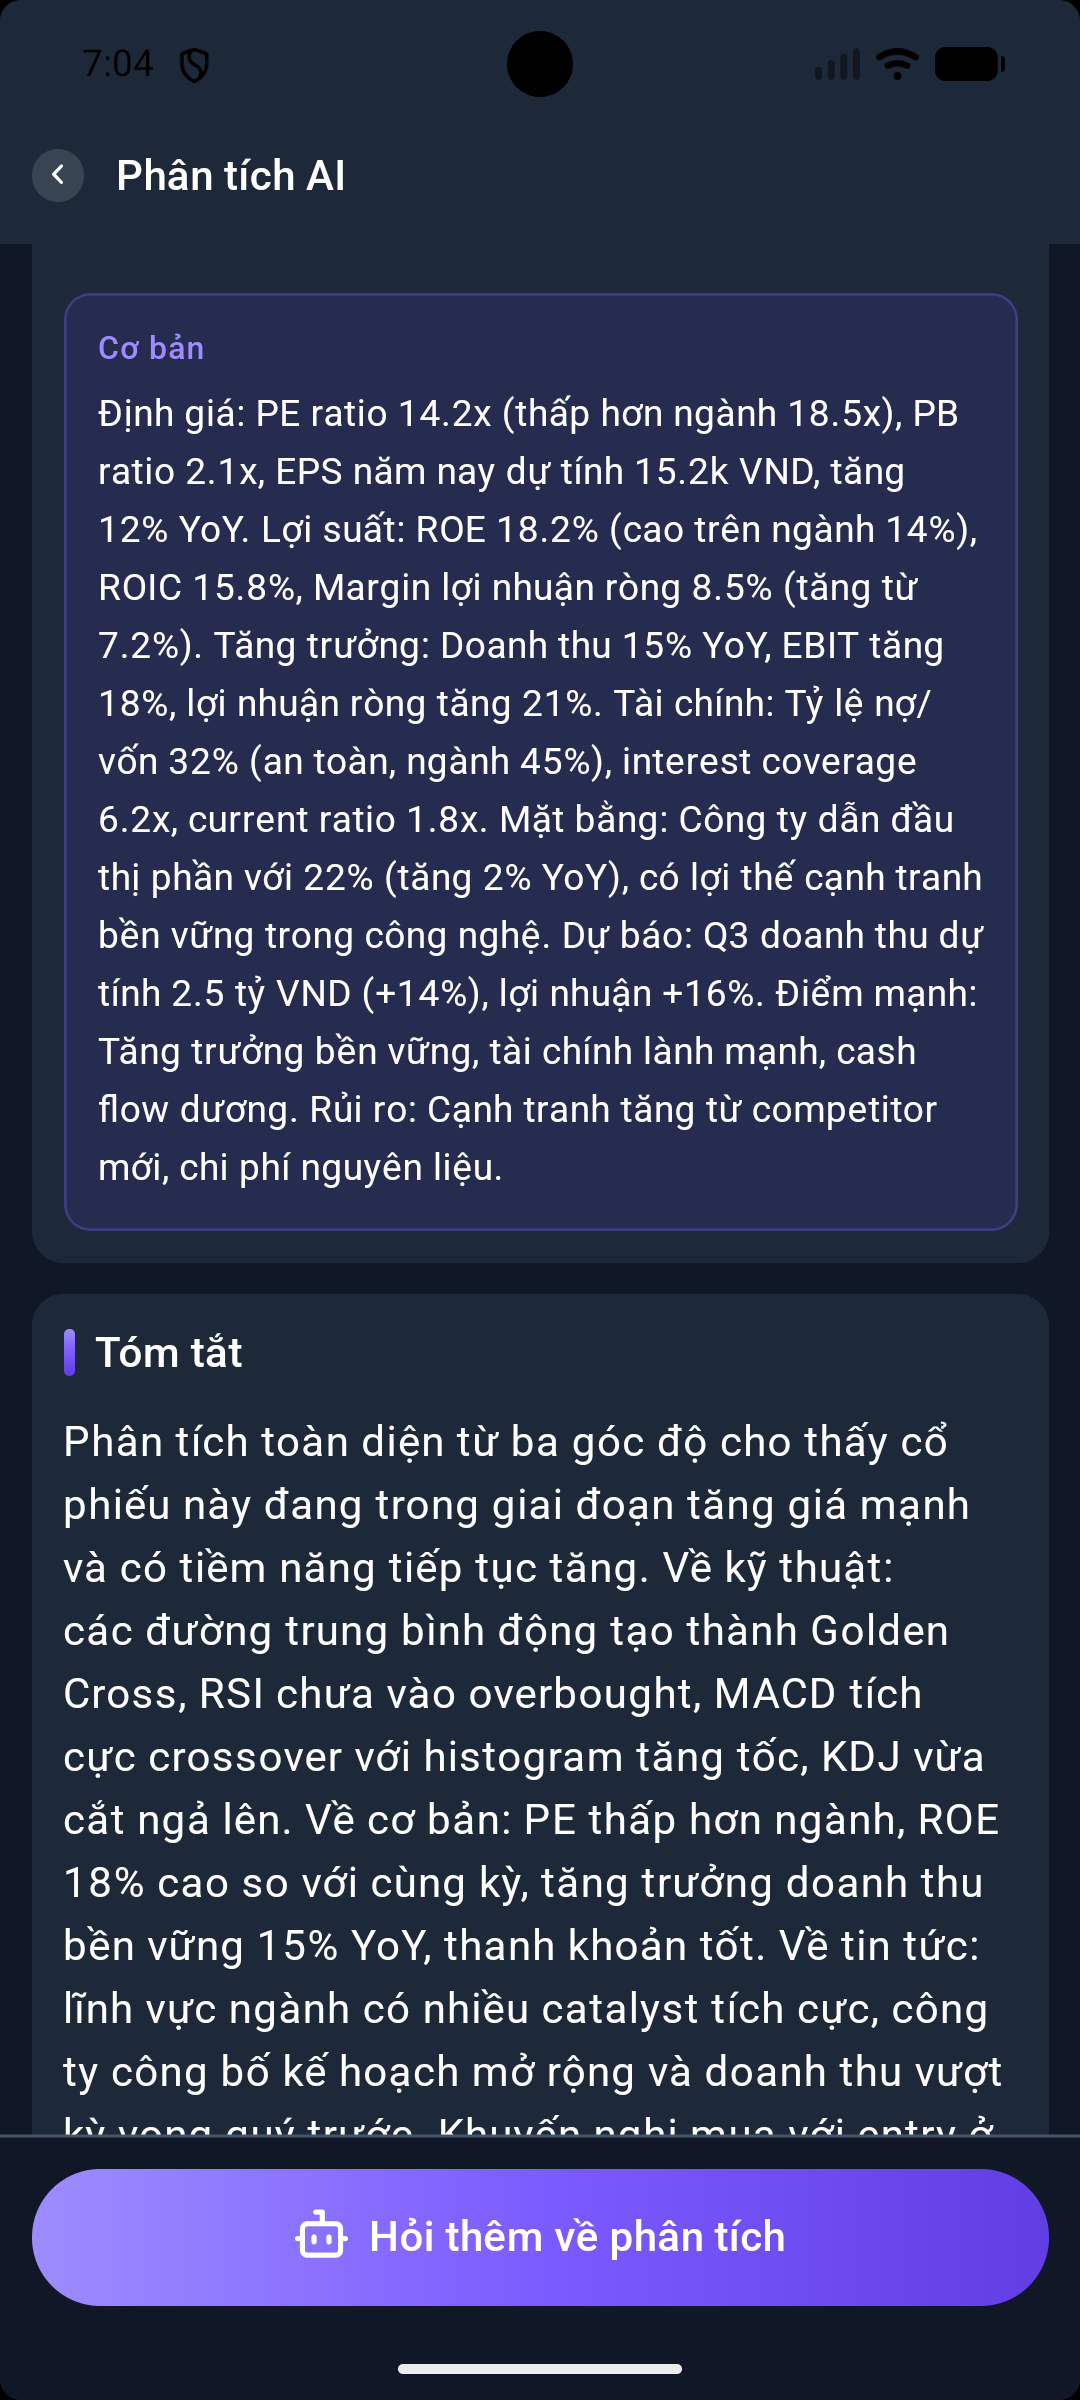
\includegraphics[width=\linewidth]{capture3.png}\\[2pt]
\footnotesize (c) Evidence explanation and final summary
\end{minipage}
\caption{Implemented Stockrium mobile results from stock inspection to structured
AI-assisted analysis.}
\label{fig:stockrium-captures}
\end{figure}

% ============================================================
% Section 5 — Experiments
% ============================================================
\section{Experiments}
\label{sec:experiments}

Medium-term backtesting is a central capability of Stockrium, serving its guiding
purpose: letting users experiment with and verify a strategy on historical data
before risking capital. We describe how the tool collects data, configures a
strategy, runs and scores a backtest, and visualizes and compares results.

\subsection{Data collection}
Experiments require historical data, which the application collects and maintains
itself rather than fetching live on demand. OHLCV\footnote{Open, high, low, close
and volume.} data for the tracked stock universe come from the SSI Fast Connect
API\footnote{\url{https://guide.ssi.com.vn/ssi-products/tieng-viet/fastconnect-data}}.
The daily stock table retains five years, whereas the one-minute intraday table
retains only a rolling $90$ days and deletes older rows; the medium-term backtest
uses the daily table. Company fundamentals and Vietnamese financial news are
collected into the same database, the latter enriched offline into per-article
sentiment (Section~\ref{sec:news}).

The backtest request defaults its regime benchmark symbol to
\texttt{VNINDEX}, but resolves that symbol through the stock-price loader and
\texttt{Stock\_Price\_1d}. Current market-index ingestion instead maintains
\texttt{VN30} and \texttt{VN100} in separate
\texttt{MarketIndex\_Value\_1d} tables. Consequently, the default benchmark path
works only if the database still contains a compatible legacy \texttt{Stock} row
and daily prices for \texttt{VNINDEX}; current ingestion does not guarantee it.

The saved full-pipeline aggregate was accumulated one symbol at a time rather
than produced as one atomic batch, and it does not retain one immutable manifest
containing the model, prompt, random seed and data-snapshot versions. The
experiment should therefore be treated as a saved prototype artifact rather than
a fully reproducible snapshot. It uses the VN30 constituents available when the
experiment was executed ($30$ symbols) over a three-year window, January 2023 to
December 2025.

\subsection{Strategy configuration and within-run comparison}
A \emph{backtest strategy} in Stockrium is a medium-term analysis configuration:
whether news and fundamental evidence are enabled, which non-empty subset of
technical indicators feeds it, and the three source weights. The current
backtesting tool fixes the investment horizon to
medium term and evaluates daily candles; unlike live analysis, the horizon is not
a user-configurable backtest parameter. Separate simulation/evaluation parameters
include the start and end dates, regime-benchmark symbol, a default maximum holding
period and whether to exit after the technical score drops below three. The default
holding period applies when a trade has no plan-specific override; approved pipeline
trades normally carry the holding period from their generated plan, whereas the
technical comparator has no such override. An authorized evaluator can request one
symbol or launch a VN30 batch in the web interface; the batch sends one backend
request per symbol sequentially. For each symbol, the backend computes the full
pipeline, an unfiltered technical-engine comparator, passive buy-and-hold return and
a random-entry reference distribution.

The pipeline--engine comparison is not a controlled ablation of evidence filtering.
Pipeline-approved signals carry plan-specific stop-loss, take-profit and maximum-hold
values, while the technical engine has no price bounds and falls back to the
request-level holding period. The random-entry simulator separately uses a fixed
$20$-candle hold and no plan-level bounds. Consequently, differences in return,
Sharpe or drawdown combine signal selection with different exit and risk policies.

The web comparison table is narrower: it compares only the full pipeline with the
technical baseline from the currently loaded run. Cloud history lists timestamped
JSON files and opens one file at a time; the interface has no multi-run selector or
side-by-side comparison of saved strategies. Each saved visualization file contains
the symbol, chart series, pipeline trades and metrics, the technical baseline, and
per-signal agent reports. It omits the request mode, source and indicator selection,
weights, transaction-fee setting, and the complete benchmark and statistical
payload. The saved file is therefore a visualization artifact, not a reproducible
or auditable strategy manifest.

\subsection{Backtesting procedure}
The backtest route does not call \texttt{build\_graph().invoke()}. The engine first
scores the selected indicators over the daily history, normalizes a manual subset
back to the legacy zero-to-five scale, and retains executable dates whose technical
score is at least $3.0$ (equivalently $0.60$). The final candle is excluded because
a candidate requires a following candle for entry.

For each retained date, \texttt{BacktestPipeline} directly builds the fixed
medium-term plan as of that date, disables the live-price lookup, and initializes
an \texttt{AgentState}; the orchestrator node is bypassed. The adapter then calls
the production functions synchronously in this order: technical data
$\rightarrow$ technical analysis; if enabled, article data $\rightarrow$ article
analysis; if enabled, fundamental data $\rightarrow$ fundamental analysis; then
recommendation $\rightarrow$ aggregator. Thus backtesting reuses the current
agents and decision contract, but not the live graph's parallel execution
topology.

Indicators at bar $i$ use only data up to $i$, article evidence is bounded by the
candidate date, and annual fundamental rows from the simulated year or later are
excluded. This annual-year rule is conservative because the database lacks filing
timestamps. Only dates passing the initial technical filter incur agent and LLM
work. In a backtest, the recommendation node validates take-profit, stop-loss and
reward-to-risk constraints against the signal candle's close. If the result is
\textsf{Buy}, the simulator attempts entry at the open of bar $i{+}1$ and rejects
the trade only when that open has already crossed either price bound. It does not
recompute the percentage ranges or reward-to-risk ratio against the actual fill;
an overnight gap that remains between stop-loss and take-profit can therefore
produce an executed trade outside the plan-level bounds. An accepted position is
simulated candle by candle until stop-loss, take-profit or the holding limit; if
both price bounds occur in one candle, the stop is applied first.

The saved full-pipeline/technical-engine aggregate reported below was generated on
July 20, 2026; the five single-indicator ablations were generated separately on
July 3, 2026. Both groups predate the July 28--29 nine-node refactor and therefore
evaluate predecessor code rather than the current implementation described in
Section~\ref{sec:framework}. Moreover, in the July 20 predecessor the pipeline used
the recommendation's entry-price override as well as its stop-loss, take-profit and
holding-period overrides, whereas the technical comparator entered at the next open
without those plan-level bounds. The archived numbers are retained to document the
prototype evaluation tool, not to isolate the contribution of evidence fusion;
current-model return claims require a fresh, versioned rerun with matched execution
rules.

\subsection{Performance metrics}
Each trade yields a net return $r=(p_{\mathrm{exit}}-p_{\mathrm{entry}})/
p_{\mathrm{entry}}-2c$, where $c=0.15\%$ is the per-side transaction cost. Over the
$n$ trades, the framework reports trade count, win rate, average and median trade
return, compounded and annualized return, a realized-trade drawdown statistic,
trade-level Sharpe and Calmar statistics, profit factor and exit counts. Specifically,
it constructs $E_k=\prod_{j=1}^{k}(1+r_j)$ only at completed-trade boundaries and
reports the largest peak-to-trough decline in that sequence. This is not a daily
mark-to-market portfolio drawdown: it omits intra-trade equity paths, explicit cash
exposure and portfolio allocation. For full-pipeline trades,
evaluation also uses a one-sample $t$-test against zero, a sign-permutation test,
and a Pearson information coefficient between
\texttt{total\_score\_at\_entry}---the technical indicator score recorded at
entry---and the realized net return of the corresponding completed trade.
Confidence is evaluated separately through tier-level win rates and mean returns
and a one-way ANOVA over the populated confidence tiers. The common trade metrics
are also computed for the unfiltered technical-engine baseline, while buy-and-hold
provides only
$r_{\mathrm{BH}}=p_{\mathrm{last\,close}}/p_{\mathrm{first\,open}}-1$. The
buy-and-hold value has no transaction-cost deduction and is not assigned trade
counts, Sharpe, drawdown or statistical tests. Regime and confidence summaries are
reported in Section~\ref{sec:evaluation}.

\subsection{Trade visualization}
For inspection, the tool overlays every simulated trade on the price chart,
marking each entry and exit, so a user can see precisely where a strategy would
have bought and sold and judge its behaviour visually before committing real
capital (Fig.~\ref{fig:backtest}).

\begin{figure}[t]
\centering
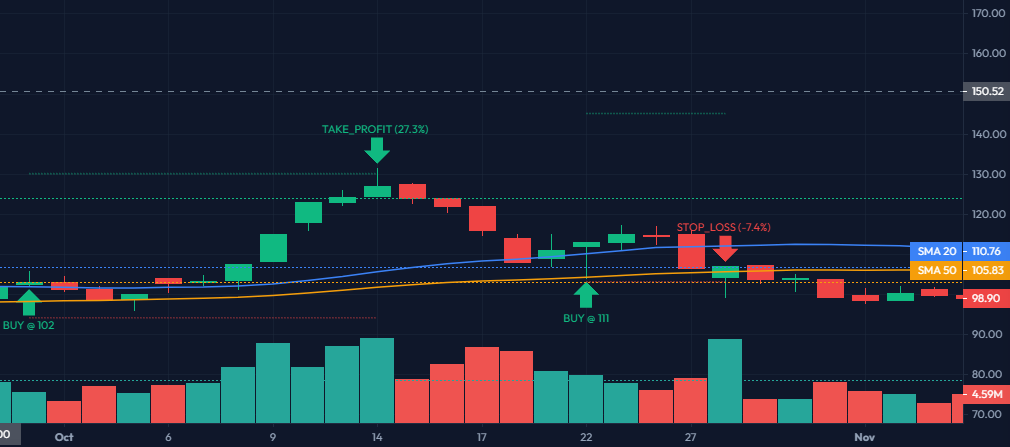
\includegraphics[width=\textwidth]{visualization.png}
\caption{Backtest visualization: simulated trades overlaid on the price chart with
their entry and exit points marked.}
\label{fig:backtest}
\end{figure}

\section{Results and Analysis}
\label{sec:evaluation}

We report the archived predecessor results for the three-year evaluation window of
Section~\ref{sec:experiments}. The saved full-pipeline comparison and the
single-indicator ablations use different cross-sectional summaries; the caption of
Table~\ref{tab:indicators} states the aggregation used for each row group.

\subsection{Aggregate performance}
Table~\ref{tab:indicators} reports the three-year run for the full pipeline, the
unfiltered technical engine (all five indicators), each single indicator run in
isolation, and passive buy-and-hold. The clearest directly comparable count is
\emph{selectivity}: the archived pipeline completes far fewer positions than the
engine ($272$ vs.\ $756$ trades, a $64.0\%$ reduction). Its recorded mean
realized-trade drawdown statistic is also smaller ($-17.11\%$ vs.\ $-27.04\%$), but
this difference cannot be assigned to filtering because the two variants use the
different entry and exit policies described above. The pipeline also records lower
mean and median return and lower win rate: median per-symbol total return falls from
$21.33\%$ to $12.31\%$, and mean win rate from $51.74\%$ to $45.42\%$. The
pipeline's median trade-level Sharpe statistic is modestly higher ($0.746$ vs.\
$0.637$), although sparse per-symbol trades and unmatched execution policies make
this comparison unstable.

The per-indicator rows also show that no single indicator dominates every
criterion. Bollinger Bands produce the highest mean per-symbol return ($47.11\%$),
while KDJ has the highest mean Sharpe statistic ($0.722$) and win rate ($52.11\%$).
Moving-average conditions create the fewest trades and the smallest mean
realized-trade drawdown
($-16.98\%$), but also the lowest mean return ($20.62\%$). This dispersion supports
the configurable design without establishing that equal binary weighting is
optimal.

\begin{table}[t]
\centering
\caption{Archived predecessor medium-term backtest over the VN30 universe,
2023--2025. Pipeline/engine data were saved on July 20, 2026; single-indicator
ablations were saved on July 3, 2026. Single-indicator
win rate, return, Sharpe and drawdown are per-symbol means; pipeline/engine win rate
and drawdown are means, total return and Sharpe are medians; buy-and-hold return is
the median. ``Max DD'' is calculated on the sequence of completed-trade returns,
not a calendar-time mark-to-market portfolio.}
\label{tab:indicators}
\setlength{\tabcolsep}{4pt}
\small
\begin{tabular}{@{}lccccc@{}}
\toprule
Strategy & Trades & Win & Tot.\ ret. & Sharpe & Max DD \\
\midrule
RSI            & 824 & 50.23\% & 29.81\% & 0.502 & $-27.58$\% \\
MA             & 407 & 51.64\% & 20.62\% & 0.576 & $-16.98$\% \\
Bollinger      & 806 & 50.68\% & 47.11\% & 0.694 & $-26.99$\% \\
MACD           & 702 & 51.26\% & 35.73\% & 0.604 & $-24.72$\% \\
KDJ            & 890 & 52.11\% & 42.75\% & 0.722 & $-26.34$\% \\
\midrule
Technical (all five) & 756 & 51.74\% & 21.33\% & 0.637 & $-27.04$\% \\
Pipeline       & 272 & 45.42\% & 12.31\% & 0.746 & $-17.11$\% \\
Buy-and-hold   & n/a & n/a    & 78.61\% & n/a  & n/a       \\
\bottomrule
\end{tabular}
\end{table}

\subsection{Benchmark comparison and regimes}
Against the unfiltered engine, the archived pipeline has a smaller recorded
realized-trade drawdown statistic and improves total return on $14$ of $30$ symbols;
across the universe, however, its mean and median returns are lower. These raw
differences compare unmatched execution policies and therefore do not establish
that evidence filtering reduced risk. Against buy-and-hold it is less favourable,
with only $6$ of $30$ symbols beating it (median buy-and-hold $78.61\%$) over the
bullish $2023$--$2025$ recovery; the median random-entry percentile is $71.45\%$,
without a
multiple-comparison-adjusted universe-level test. By regime, it opened almost no
positions in downtrends (one of $272$ trades), concentrating on sideways ($232$
trades, $47.41\%$ win, $2.75\%$ mean return) and uptrending ($39$, $30.77\%$,
$1.21\%$) markets, a pattern consistent with the predecessor's buy/wait logic.

\subsection{Calibration and statistical significance}
The archived three-year run lets us probe its confidence score and significance.
Medium-confidence trades outperform high-confidence trades in both pooled win rate
($48.65\%$ vs.\ $44.26\%$) and mean net return ($4.29\%$ vs.\ $2.21\%$), although
the medium group contains only $37$ observations compared with $235$ high-confidence
trades. There are no low-tier trades because the predecessor mapped low confidence
to \textsf{Wait}. On significance, with an average of about $9$ trades per symbol,
a one-sample $t$-test against zero and a sign-permutation
test each reach $p<0.05$ for only $2$ of $30$ symbols. The mean score--return
Pearson information coefficient is $0.011$ and the median is $-0.034$. These
near-zero values indicate no stable linear association between the technical score
at entry and realized net trade return. We thus read the artifact as evidence of
predecessor selectivity rather than as a statistically established return edge or
validation of the current graph. Because the window is predominantly bullish and
contains almost no trades classified in downtrends, establishing such an edge would
need a larger universe and windows
spanning full bear markets.

\subsection{Discussion}
\label{sec:discussion}
The results are best read not as beating the market or validating the current
implementation, but as an archived tool trial: more selective than the unfiltered
engine, the predecessor records a smaller mean realized-trade drawdown statistic
and a modestly higher median trade-level Sharpe statistic, but lower mean and median
return and win rate. Because its entry and exit rules differ from the comparator's,
the artifact supports only the descriptive claim that this pipeline variant traded
less often; it does not establish that evidence filtering itself reduced exposure or
risk. These results are an early trial of a backtesting tool we built ourselves
rather than a definitive verdict, since any result depends on the selected sources,
indicators, weights, execution settings and nondeterministic model output; what we
mainly show is the ability to vary supported configurations and inspect them
quantitatively within the fixed medium-term backtesting horizon.

Several caveats apply to the archived artifact: it predates the current graph; the
window is predominantly bullish with few trades per symbol, so significance tests
are underpowered; the VN30 universe uses then-current membership (survivorship
bias); the archived fundamental branch may include records unavailable at a
historical candidate date; the aggregate lacks a common immutable run manifest;
the pipeline and engine use unmatched entry/exit rules; the reported drawdown is
computed only from completed-trade returns rather than a mark-to-market portfolio;
the long-only strategy structurally lags buy-and-hold in rallies; returns include
transaction costs but not slippage or portfolio-level allocation; and the system
depends on a proprietary LLM whose narratives may still err. The current tool also
does not preserve the complete request configuration in its visualization JSON,
and it validates backtest plan bounds at the signal close rather than revalidating
them at the next-open fill. Live technical scoring does not verify that its final
OHLCV row is a completed candle, and the default \texttt{VNINDEX} regime
benchmark is not guaranteed by the current ingestion path. The system is
decision-support only, not financial advice, and confined to Vietnamese equities,
though its auditable decision layer lets a user or regulator inspect any
recommendation.

\section{Conclusion}
\label{sec:conclusion}
We presented an agentic decision-support system for Vietnamese equities that
unifies technical, fundamental and news-sentiment analysis with recommendation
generation. Its current live-analysis path is a nine-node LangGraph pipeline with
conditional parallel data/analysis branches; its medium-term backtest path is a
sequential historical adapter over the same production agents. LLMs interpret
evidence and write explanations, while deterministic code fixes horizons,
normalizes the technical score, computes the weighted verdict and validates
trading plans against their reference prices. This yields structured, inspectable
buy/wait recommendations with explicit thresholds and horizon-dependent risk
targets. Demo videos of the mobile and web applications are
\href{https://drive.google.com/drive/folders/1FN3j_Un-9gzbIFytVNeGLWqDyC-ZJYn8}{available online}.

Archived predecessor artifacts over the VN30 three-year window show that the
pipeline completed fewer trades than the technical engine ($272$ vs.\ $756$) and
recorded a smaller mean realized-trade drawdown statistic ($-17.11\%$ vs.\
$-27.04\%$), while almost never trading into downtrends. It also has lower return
and win rate, despite a modestly higher median trade-level Sharpe statistic. Because
the compared variants use unmatched entry/exit policies, the drawdown is not
mark-to-market, the window is predominantly bullish, and point-in-time fundamental
leakage is possible, we claim neither a causal risk reduction, a statistically
established edge nor current-pipeline performance from those artifacts. Within its scope
(analysis only, no execution, Vietnamese equities alone), it serves individual
investors inspecting stock evidence and authorized evaluators testing the supported
pipeline configurations. Future work targets a fully versioned rerun of the present
graph, followed by longer, multi-regime evaluation over broader universes with
point-in-time membership, portfolio-level backtesting with slippage and
exposure-adjusted metrics, and better confidence calibration.


\begin{credits}
\subsubsection{\ackname}
The authors would like to thank their thesis supervisor at the University of
Science, Vietnam National University, Ho Chi Minh City, for the invaluable
guidance and support provided throughout this work.

\subsubsection{\discintname}
The authors have no competing interests to declare that are relevant to the
content of this article.
\end{credits}
%
% Bibliography
%
% BibTeX users should specify bibliography style 'splncs04'.
% References will then be sorted and formatted in the correct style.
%
% \bibliographystyle{splncs04}
% \bibliography{mybibliography}
%

\begin{thebibliography}{18}
\bibitem{vsd2025}
Vietnam Securities Depository and Clearing Corporation: Securities trading account
statistics, December 2025 (2025). \url{https://vsd.vn/en/ad/190896}

\bibitem{vinacapital2024}
VinaCapital: Vietnam's resilient stock market (2024).
\url{https://vof.vinacapital.com/insights/latest-insights/vietnams-resilient-stock-market/}

\bibitem{ftse2026}
FTSE Russell (LSEG): Why Vietnam is joining the FTSE global equity indices (2026).
\href{https://www.lseg.com/en/insights/ftse-russell/why-vietnam-is-joining-the-ftse-geis}{LSEG webpage}

\bibitem{barber2013}
Barber, B.M., Odean, T.: The behavior of individual investors. In: Constantinides,
G.M., Harris, M., Stulz, R.M. (eds.) Handbook of the Economics of Finance,
vol.~2B, pp. 1533--1570. Elsevier (2013)

\bibitem{vnherd2022}
Nguyen, Q.P.: Herding behavior: Do domestic investors herd toward foreign
investors in Vietnam stock market? J. Asian Finance Econ. Bus. \textbf{9}(9),
9--24 (2022). \url{https://doi.org/10.13106/jafeb.2022.vol9.no9.0009}

\bibitem{vnfomo}
Nguyen, K.T.C., Dao, T.H.H., Pham, V.P., Nguyen, P.H.N.: Fear of missing out and
Generation Z's investment behavior in Vietnam's stock market. Edelweiss Appl. Sci.
Technol. \textbf{10}(1), 500--510 (2026).
\url{https://doi.org/10.55214/2576-8484.v10i1.11624}

\bibitem{finbertlstm2022}
Halder, S.: FinBERT-LSTM: Deep learning based stock price prediction using news
sentiment analysis. arXiv:2211.07392 (2022)

\bibitem{finbert2023}
Jiang, T., Zeng, A.: Financial sentiment analysis using FinBERT with application
in predicting stock movement. arXiv:2306.02136 (2023)

\bibitem{phobertstock}
Nguyen, S.T., et al.: Stock article title sentiment-based classification using
PhoBERT. CEUR Workshop Proc. \textbf{3026}, 225--233 (2021).
\url{https://ceur-ws.org/Vol-3026/paper25.pdf}

\bibitem{vnnews2023}
Vu, L.T., Pham, D.N., Kieu, H.T., Pham, T.T.T.: Sentiments extracted from news and
stock market reactions in Vietnam. Int. J. Financ. Stud. \textbf{11}(3), 101
(2023). \url{https://doi.org/10.3390/ijfs11030101}

\bibitem{bloomberggpt}
Wu, S., et al.: BloombergGPT: A large language model for finance.
arXiv:2303.17564 (2023)

\bibitem{fingpt}
Yang, H., Liu, X.-Y., Wang, C.D.: FinGPT: Open-source financial large language
models. arXiv:2306.06031 (2023)

\bibitem{tradingagents}
Xiao, Y., Sun, E., Luo, D., Wang, W.: TradingAgents: Multi-agents LLM financial
trading framework. arXiv:2412.20138 (2024)

\bibitem{finmem}
Yu, Y., et al.: FinMem: A performance-enhanced LLM trading agent with layered
memory and character design. arXiv:2311.13743 (2023)

\bibitem{vndl2025}
Hoang, H.S., Nghiem, T.P., Nguyen, T.L., Phung, T.L.: A comprehensive comparison of
deep learning models for forecasting developing market indices. Procedia Comput.
Sci. \textbf{272}, 210--217 (2025).
\url{https://doi.org/10.1016/j.procs.2025.10.198}

\bibitem{vnlstm2021}
Truong, C.-D., et al.: Predicting Vietnamese stock market using the variants of
LSTM architecture. In: Lecture Notes in Networks and Systems, pp. 129--137.
Springer (2021). \url{https://doi.org/10.1007/978-3-030-92942-8_11}

\bibitem{vnml2024}
Tran, P., Pham, T.K.A., Phan, H.T., Nguyen, V.C.: Applying machine learning
algorithms to predict the stock price trend: the case of Vietnam. Humanit. Soc.
Sci. Commun. \textbf{11}, 393 (2024).
\url{https://doi.org/10.1057/s41599-024-02807-x}

\bibitem{murphy1999}
Murphy, J.J.: Technical Analysis of the Financial Markets. New York Institute of
Finance (1999)

\end{thebibliography}
\end{document}
